\chapter{The Atacama Cosmology Telescope: point source analysis of beams for DR6}
\label{ch:actbeams}

\section{\label{sec:intro}Introduction}
\setcounter{footnote}{0}

The Atacama Cosmology Telescope (ACT) is a 6\,m off-axis Gregorian telescope located at an altitude of 5190\,m in the Atacama Desert of northern Chile. It is designed for millimeter wavelength observations of the cosmic microwave background (CMB) at arcminute resolution.  The telescope and receiver are described in \cite{fowler_2007} and \cite{thornton_2016} respectively. 

This paper describes the ACT point source beams for its sixth data release, referred to as DR6. This data release includes temperature and polarization data collected by ACT between 2017 and 2020, covering XXX regions of the sky spanning roughly 18,000?? deg$^2$, in frequency bands centered on 98 and 220 GHz \citep{thornton_2016}.

The DR6 data were obtained using three dichroic detector arrays, PA4, operating at 150 and 220 GHz, PA5, operating at 98 and 150 GHz, and PA6, operating at 150 and 220 GHz.  The three array positions are not identical optically. Each year of data is referred to as a season (S17--S20).  The DR6 data products and some of their analyses are presented in  \cite{XXX}, \cite{aiola_2020},... 

Quantifying the beam of the telescope determines the instrument's response at various angular scales.  For this reason, understanding the telescope beam and its uncertainty is critical for achieving the science goals of ACT.  For example, a false characterization of the beam can mimic cosmological affects on the CMB power spectrum from the spectral index of inflation $n_s$.  Therefor, in order to achieve the science goals set out by ACT, characterization of the instrument beam is crucial.

Previous work to characterize the ACT instrument beam have done so with co-added planet maps (~\cite{hasselfield_atacama_2013,louis_2017,naess_2014}).  Here, we present a novel technique to characterize the instrument beam with map data, which we refer to as "stacking" of the point-sources in a map's catalog.  This work provides a detailed recipe for characterizing an instrument's beam using full map data, which we apply to the ACT DR6 maps.

The paper is organized as follows. 
In \S\ref{sec:obs} we describe the observations and catalog used to stack point sources and characterize the ACT beams.  In \S\ref{sec:stack} we explain the stacking process, starting from an input map and producing a stacked beam profile.  In \S\ref{sec:sim_pipe} we describe the steps of the map simulation pipeline, then going from simulated point-source maps to a model of the ACT beams and their covariance.  In \S\ref{sec:results} we present the results from the stacking method, including the stacked temperature to polarization leakage, and the temperature beam radial profiles.  Finally, in \S\ref{sec:disc} we discuss assumptions made in the analysis and future directions for ACT beam characterization.

\section{Observations}
\label{sec:observations}
\textcolor{red}{Adri:}
\label{sec:obs}
\begin{itemize}
    \item description of CMB maps
    \item from 2017-2021 in these f bands and this patch of the sky
    \item ML vs. Special point source description
\end{itemize}
To characterize the telescope's beam to sufficiently large angles, observations of high signal-to-noise point-source measurements are required.  In past seasons of ACT data releases, planets served as the best candidates for beam characterization of the telescope~\cite{Lungu_2022}.  Specifically, observations of Uranus achieve adequate signal-to-noise without exceeding the dynamic range of the instrument and thus has been treated as a point source.
\begin{figure*}
\vspace{1em}
    \centering
    \includegraphics[width=\textwidth]{Figures/pt_src_dist.png}
    \caption{Distribution of the total number of point sources that were in the catalog (faded colors) and ultimately became part of the final beam analysis (solid colors) for all arrays combined, shown by observing seasons from 2017--19.
    }
    \label{fig:ptsrc_select}
    \vspace{1em}
\end{figure*}
\section{Methods}
\label{sec:stack}
Here we walk through the stacking process from input map to beam profile.  

\subsection{Point-source Selection}
\label{subsec:ptsrc_sel}
Prior to stacking, we characterize each beam to determine whether they are suitable for stacking.  The number of point sources used for the beam analysis versus the total number of point sources in the catalog is shown in Figure~\ref{fig:ptsrc_select}.

\subsubsection{Select on Catalog}
\label{subsubsec:cat_sel}
The full map for a specified PA and F-band is masked with a "\text{red}{BN Bottom cut, replace name}", since we want to use the same part of the map which we also use for cosmology.  From the point-source catalog, we obtain a list of ras and decs of point-sources in the map.  However, it is not a given that each point-source from the catalog appears on our map, so we reject any coordinates which fall outside the boundary of the input map $m$. 
Additionally, we select only point synchotron sources, such that we stack over individual point sources rather than galaxy clusters.  When stacking polarized beams, we restrain the point sources to a polarization fraction of below 10\% such that we are not dominated by highly polarized sources. Once the selection is complete, the geometry of the stamp is defined to be $40\arcmin$($30\arcmin$) wide at a $XX\arcmin$ resolution for the F090 and F150(F220) bands.  The region must be large enough such that the stamp will include side-lobes features, but resolved enough to make out the main beam profile.

\subsubsection{Select on Beam Quality}
\label{subsubsec:beamqual_sel}
With the list of point-source locations on our map from the catalog, we further decide which point-sources to use in the stamp based on a stamp's individual features.  For example, we don't want to include a stamp with two point-sources, or an off-center point-source, in the stack.  To characterize the quality of a beam, each point-source is re-projected to the same geometry (as specified in the last paragraph).  A point source $p_i$ is first peak-normalized.  If the location of its highest peak, $p_{i,1}$, is outside a radius of $0.5\arcmin$, $p_i$ is assumed to be off-centered and is discarded.  

We next want to determine if the stamp has two point-sources or just one.  To do so, we find the second-highest amplitude in the stamp and assume this to be the "second"-peak, $p_{i,2}$.  If the amplitude of $p_{i,2}$ is within 10\% of the average stamp value (outside the radius $r=\sqrt{8\ln{2}}\,\sigma\times 2/3$), it is assumed to be dominant, and the point source $p_i$ is discarded.

Figure~\ref{fig:ptsrc_select} shows the number of point sources used in each band and PA from the catalog.  We note that the F090 map stacks included the greatest number of point sources, since the beams are larger and therefore take up a larger area of the stamp's area.  Because the F220 beams are much smaller in beam width, we constrain stamps in this band to a radius of $15^{\circ}$, while the F090 and F150 stamps are at a radius of $30^{\circ}$.

\begin{figure*}
    \centering
    \includegraphics[width = \textwidth]{Figures/ptsrc_map.png}
    \caption{Spatial distribution of point sources from catalog(grey) and used in stacking(colored).  The colorbar shows the flux of the special(ML) sources, which are plotted as triangles(circles).}
    \label{fig:ptsrc_map}
\end{figure*}
\subsubsection{Special vs. ML Sources}
\label{subsubsec:type_sel}
We subdivide the remaining point sources into two categories: Special and Max-Likelihood (ML) point sources.  When making the maps, as described in Section~\ref{sec:observations}, point sources are treated with the two differing methods, and thus we want to consider the two groups individually when stacking to note any differences this treatment may have caused.

The final distribution of selected beams is shown in Figure~\ref{fig:ptsrc_select}.  The F220 PA4 contains the least amount of sources due to the smaller beam size in the higher band.  This amount of point sources can be increased by reducing the stamp size of the stack, such that fewer stamps are flagged due to containing two beams in a given stamp.

\subsection{Stacking}
\label{subsec:stacking}
This section describes the stacking procedure with the selected beams.  Each stamp $s_i$ is re-projected to the same geometry prior to stacking.  Because we want our final product to be the beam of the telescope, we employ a large-scale structure removal procedure such that all we are left with is the beam.  First, we use a method we call "inpainting".  This procedure masks the center beam and fills this area with a predicted large-scale structure from information in the outer area of the stamp.  \textcolor{red}{Adri: add paragraph describing inpainting description, sentence about bias}. This returns our point-source-free stamp, $s_{i,l}$.  We then subtract $s_{i,l}$ from our original stamp, $s_i$:
\begin{equation}
    s_i^{,} = s_i - s_{i,l}
\end{equation}
The final step is weighing each stamp and stacking them together.  We employ an inverse-variance weighting, where the weight is always calculated from the intensity $I_i$ beam, and the same weight is applied the $Q_i$, $U_i$, $E_i$ and $B_i$ stamps.  The variance $\sigma^2$ is calculated between $r_{in}$ and $r_{out}$ of the stamp, where $r_{in}$ is defined as the radius where the planet profile drops below $-35$\,dB (both $s_i^{,}$ and $s_p$ peak-normalized), and $r_{out}=\frac{4}{3}r_{in}$.  The weight of the stamp $w_i$ is then the inverse variance of $I$ within $r_{in}$ and $r_{out}$.  Once the above is calculated for all stamps in the set, the stack is calculated by:
\begin{equation}
    \bar{s} = \frac{\sum_i s_i w_i }{\sum_i w_i}
\end{equation}
Figure~\ref{fig:example_maps} shows two example outputs of the stacking, for PA5 F090 and F150.  
\begin{figure}
    \centering
    \includegraphics[width=.35\textwidth]{example-image-a}
    \caption{Two examples of resulting beams from stacked point sources.  Top: PAX F090 beam and Bottom: PAX F150 beam...}
    \label{fig:example_maps}
    \vspace{1em}
\end{figure}
\subsection{Bias From Stacking}
\label{subsec:bias}
To study this bias, a set of simulated observations are processed through the stacking process.  The full simulation pipeline is described in Section~\ref{sec:sim_pipe}.
\begin{figure*}[ht!]
    \centering
    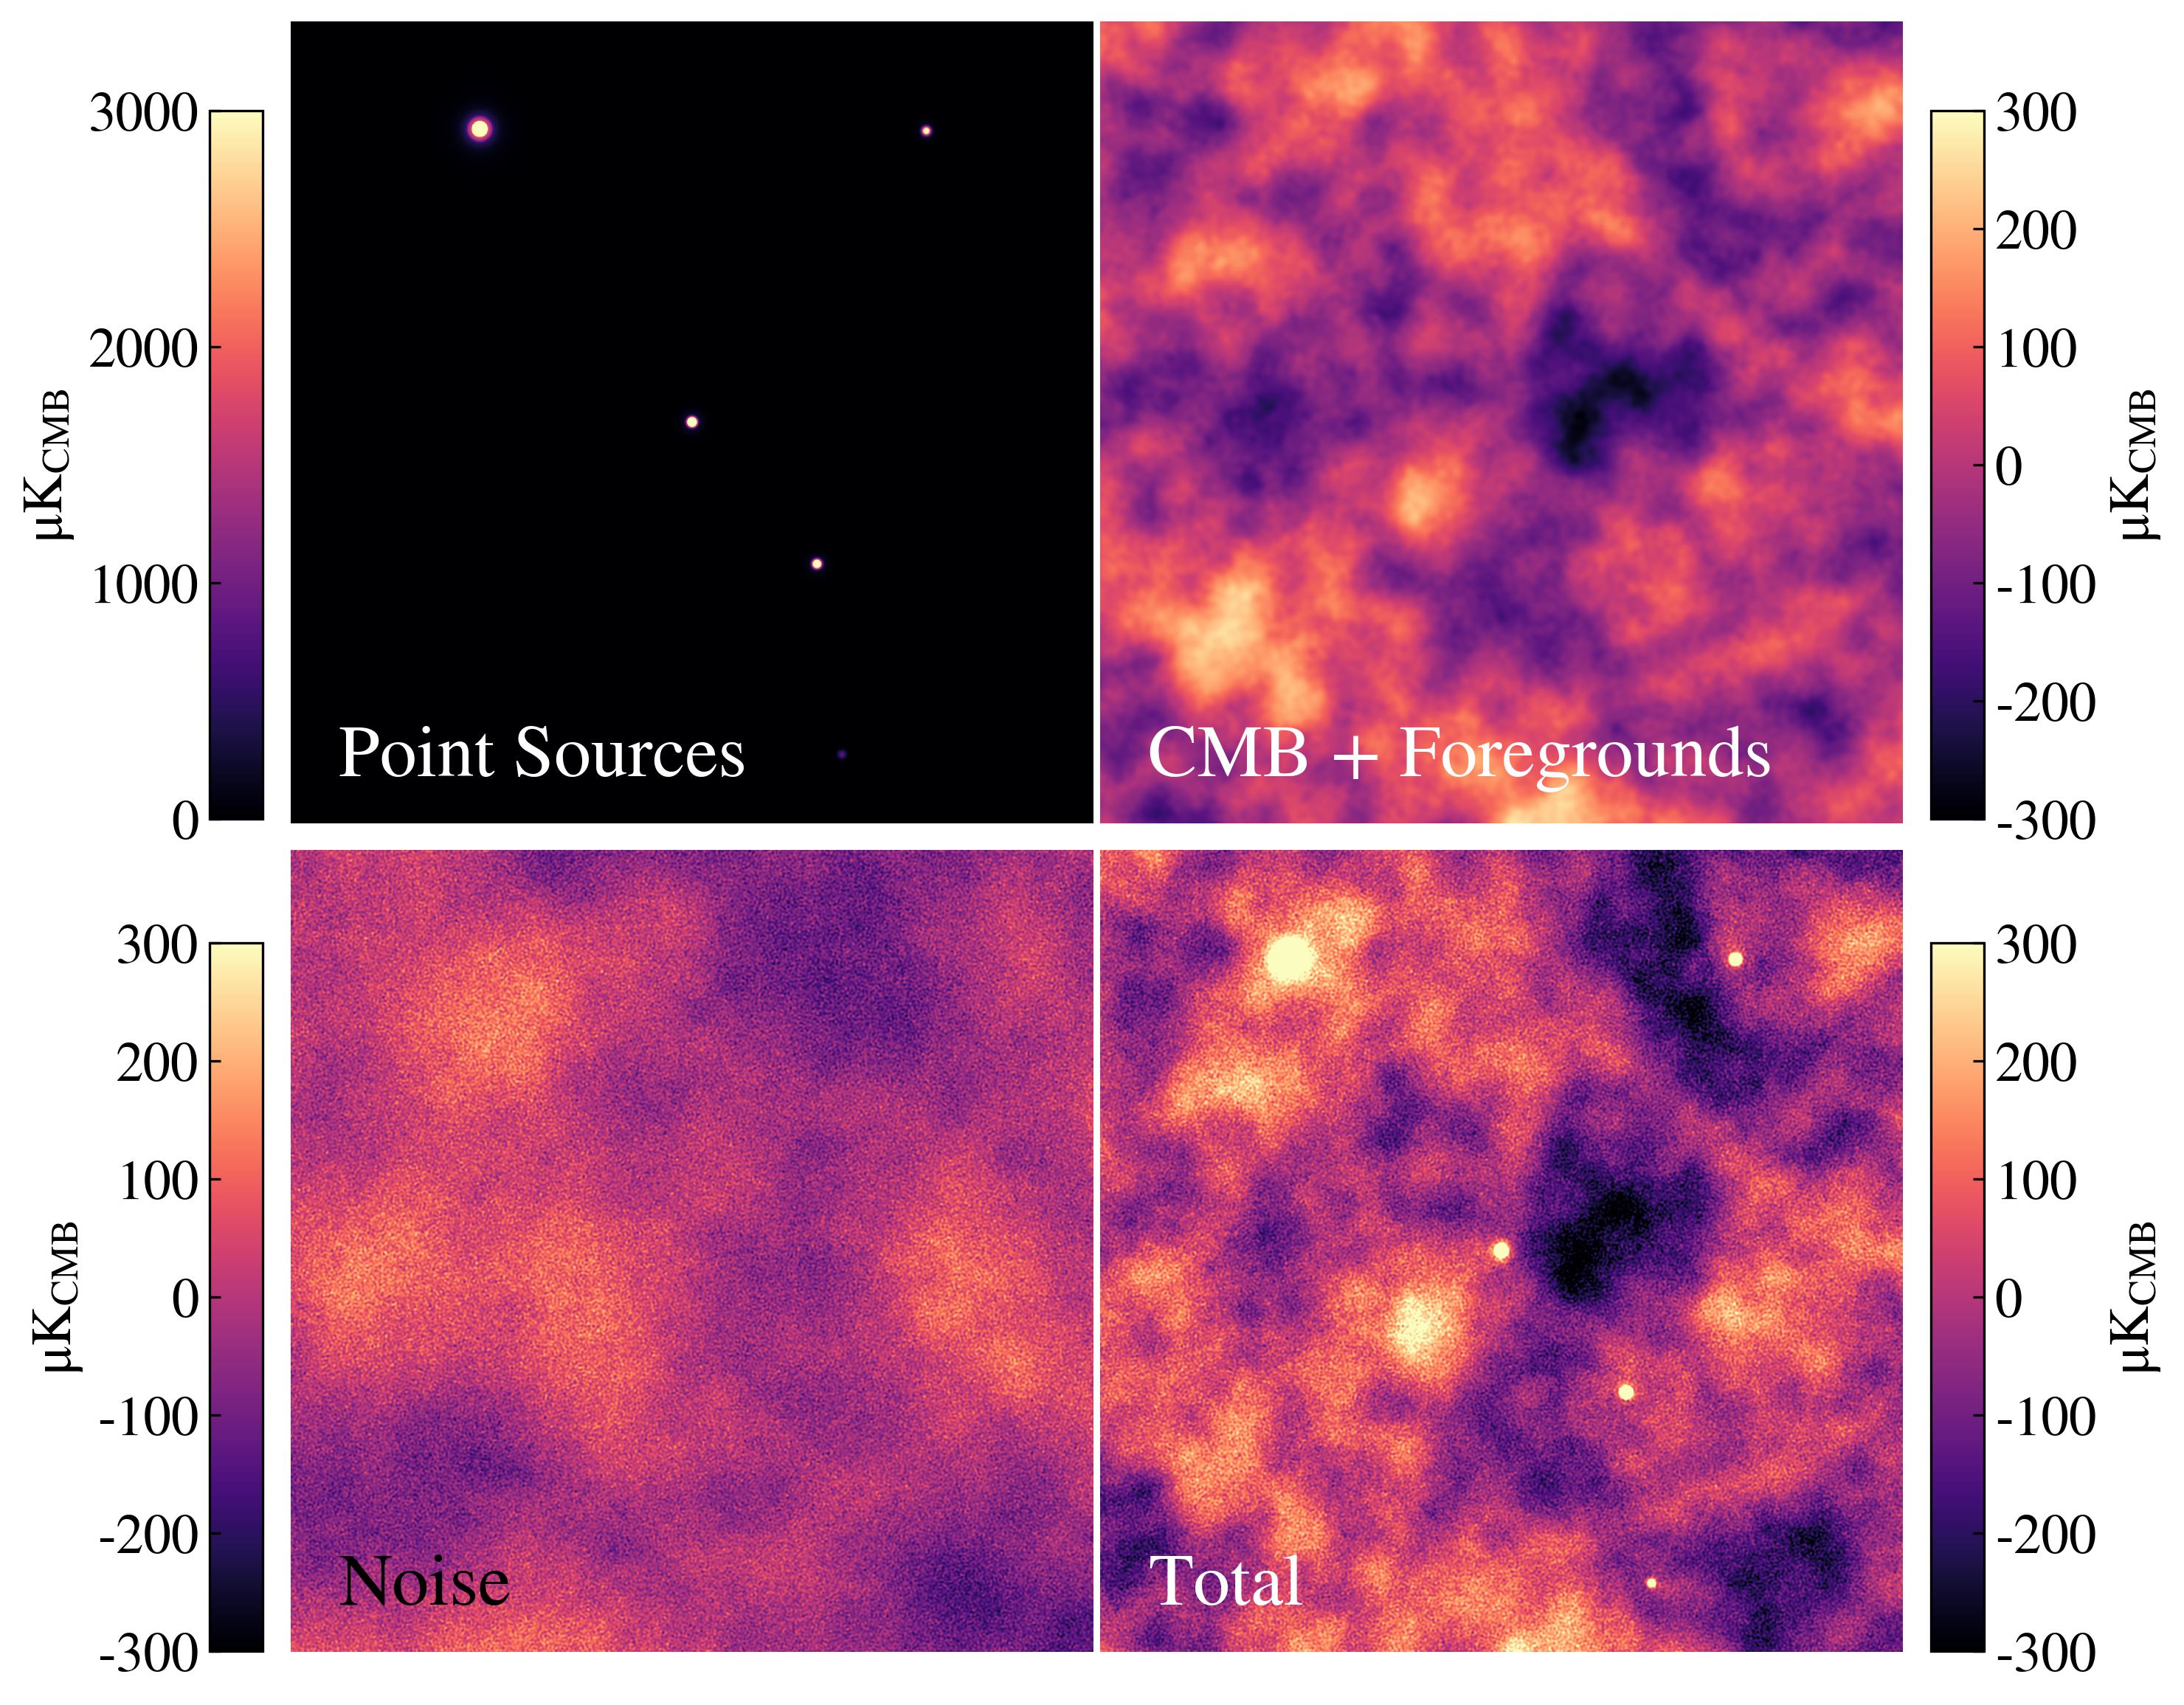
\includegraphics[width=.9\linewidth]{Figures/simmap.png}
    \caption{Example of a simulated map used to characterize the stacking bias.  This example is for PA5 in the F090, zoomed in to an area of $2\deg\times2\deg$.  Top left: Point-source map using the input catalog ra and dec coordinates.  Top right:  Simulated CMB.  Bottom left:  Simulated noise~\cite{atkins}.  Bottom right: Final simulated map after combining the previous three components.  This process is done for each PA and F-band, and repeated 100 times to estimate radial profile errors.
    }
    \label{fig:sim_map}
\end{figure*}
\begin{figure*}
    \centering
    \includegraphics[width=\textwidth]{Figures/profiles_noP_15.png}
    \caption{The average radial profile of the simulated observations for PA5 at 150 GHz, comparing the azimuthal averages of the \enquote{input} 2D beam model and the beam of the \enquote{output} stacked point sources. 
    }
    \label{fig:profiles}
\end{figure*}

\subsection{Radial Profiles}
\label{subsec:profs}
Maps are binned into a symmetrized radial profile with bins of varying width, out to a radius of 20$^{\prime}$(15$^{\prime}$) for F090 and F150(F220), independently for each detector array, and frequency band.  The bins are chosen to be logarithmic in radius.  We ultimately want to compare the stacked profiles to the planet profiles.  To do so, we first convert the planet profiles to a 2D stack matching the stamp geometry of the stacked beam.  We then radially bin the new planet profile beam with the same bins used on the stacks.

Error of the radial profiles is obtained by simulating and stacking 100 maps with the simulation pipeline described in Section~\ref{sec:sim_pipe} and Section~\ref{sec:stack}.  The covariance matrix of these 100 simulated radial profiles estimates the error of our "true" stacked profiles at each binned radius.

\subsection{Beam Window Functions}
\label{subsec:window}
In spherical harmonic space, the beam information is encoded in the harmonic transform $b_{\ell}$ and the window function $w_{\ell} = b_{\ell}^2$, which describes the instrument's response to different multipoles, $\ell$. This window function is an essential component of the DR4 power spectrum analysis in \cite{choi_2020}.

The harmonic transform $b_{\ell}$ is the Legendre transform, or more accurately the Legendre polynomial transform, of the beam radial profile:
\begin{equation}
b_{\ell} = \frac{2\pi}{\Omega}\int_{-1}^{1} B(\theta)P_{\ell}(\cos\theta)\; d(\cos\theta) \; .
\label{eq:legendre}
\end{equation}
Extension of this, introduce spin-2 ...

For small beams, such as that of ACT, this is effectively a Fourier transform. The derivation of the Legendre transform and details about how the transform is computed are presented in~\cite{Lungu_2022}.

We use $b_{\ell}$ instead of $B_{\ell}$ to indicate the division by $\Omega$, which normalizes $b_{\ell}$ to unity at $\ell = 0$ (since $P_0 = 1$). $B_{\ell} = \Omega b_{\ell}$ has units of $\mathrm{sr}$, whereas $b_{\ell}$ is dimensionless. We extrapolate the model beyond the fit radius of 10$^{\prime}$ when computing the transform.
This is necessary to capture the low-$\ell$ part of the window function, and to account for the part of the beam solid angle that is beyond the range we fit.

A subset of the beam transforms from DR6 is shown in Figure... 

\section{Simulation Pipeline}
\label{sec:sim_pipe}
An example of a simulated map (box area of $\pm1\deg$ \textcolor{red}{FIX THESE VALUES TO MATCH STAMP}) is shown in Figure~\ref{fig:sim_map}.  The four quadrants show the three main components of the simulated maps, followed by the total simulated map as the prior three are combined.
\subsection{Point Source Map Simulation}
\label{subsec:sim_ptsrc}
A point source map is simulated using the input catalog, and point source selection described in Section~\ref{subsubsec:cat_sel}.  The planet profile defines the shape of the point sources in the simulated map.  Fluxes of each point source are obtained from the catalog and normalized to beam area (steradians) and center frequency of the band (converted to mJy/sr).

The \verb|pixell.sim_objects| function takes the desired map geometry, the beam profile, and fluxes, and creates a simulated point source map.  We apply a window function to the point source map
\textcolor{red}{(pixwin = True option)}.  The result is a simulated point source map with matching point sources and map shape as the catalog and DR6 map, respectively. 

\subsection{CMB Simulation}
\label{subsec:sim_cmb}
The second component of the simulation is the CMB.  It is critical to add this to our simulation since we include a large-scale structure subtraction in our stacking, so this piece will determine any potential bias introduced during our subtraction procedure.  First, we use the ACT DR4 $C_{\ell}^{TT}$ power spectra, which covers the high $\ell$ spectrum~\cite{aiola_2020}.  This is stitched together with lower $\ell$ spectra from~\cite{YYY}.  An example patch of the CMB spectra map is shown in the top right of Figure~\ref{fig:sim_map}. 
 This simulation also contains foregrounds, which are an important contribution at high multipoles.

\subsection{Noise Simulation}
\label{subsec:sim_noise}
The third component to complete our simulated maps is noise.  The estimation of map noise is twofold: 1) an $a_{\ell,m}$ map-based noise simulation and 2) estimated noise from variance maps.

Map-based noise simulations are fully described here~\cite{}.  Noise simulation maps include atmosphere, ACT scan strategy, and a more detailed approach to model correlated instrument noise.  An individual noise simulation is used for each individual simulated map.  An example patch of the noise map is shown in the bottom left of Figure~\ref{fig:sim_map}.

The second source of noise is taken from the variance maps of the data, which we refer to as the "white noise" term.  We then splice together two noise simulations in $\ell$-space, such that the white noise term occupies the lower $\ell$ space and map-based noise dominates the high $\ell$ space.

\section{Results}
\label{sec:results}
\subsection{Main Beam}
\label{subsec:mainbeam}
This section presents the temperature profiles from stacks and compares them to the existing planet profiles from Uranus. 
\subsubsection{Profiles}
\label{subsubsec:profiles}
The stacked profiles are shown in Figure~\ref{fig:profiles}.  Each profile shows the Uranus planet profile in black, with individual arrays plotted separately.  The bottom panel shows the difference between each array's profile to the planet.
\subsubsection{Spatial Variation}
\label{subsubsec:null_mainbeam}

To study the spatial variation of point sources, we conducted a "null test" where we stacked four categories of point sources: high and low, RA and DEC.  We separate the catalog in half by considering the median RA and DEC, such that the four categories are $\text{RA}_{\text{low}}$, $\text{RA}_{\text{high}}$, $\text{DEC}_{\text{low}}$ and $\text{DEC}_{\text{low}}$. 
 Figure~\ref{fig:bells} shows the resulting window functions $B_{\ell}$ for each F-band and PA.

From this test, we find the special sources have spatial dependence where the $\text{DEC}_{\text{low(high)}}$ and $\text{RA}_{\text{high(low)}}$ match in window function, but differ from its opposite.

\begin{figure*}
    \centering
    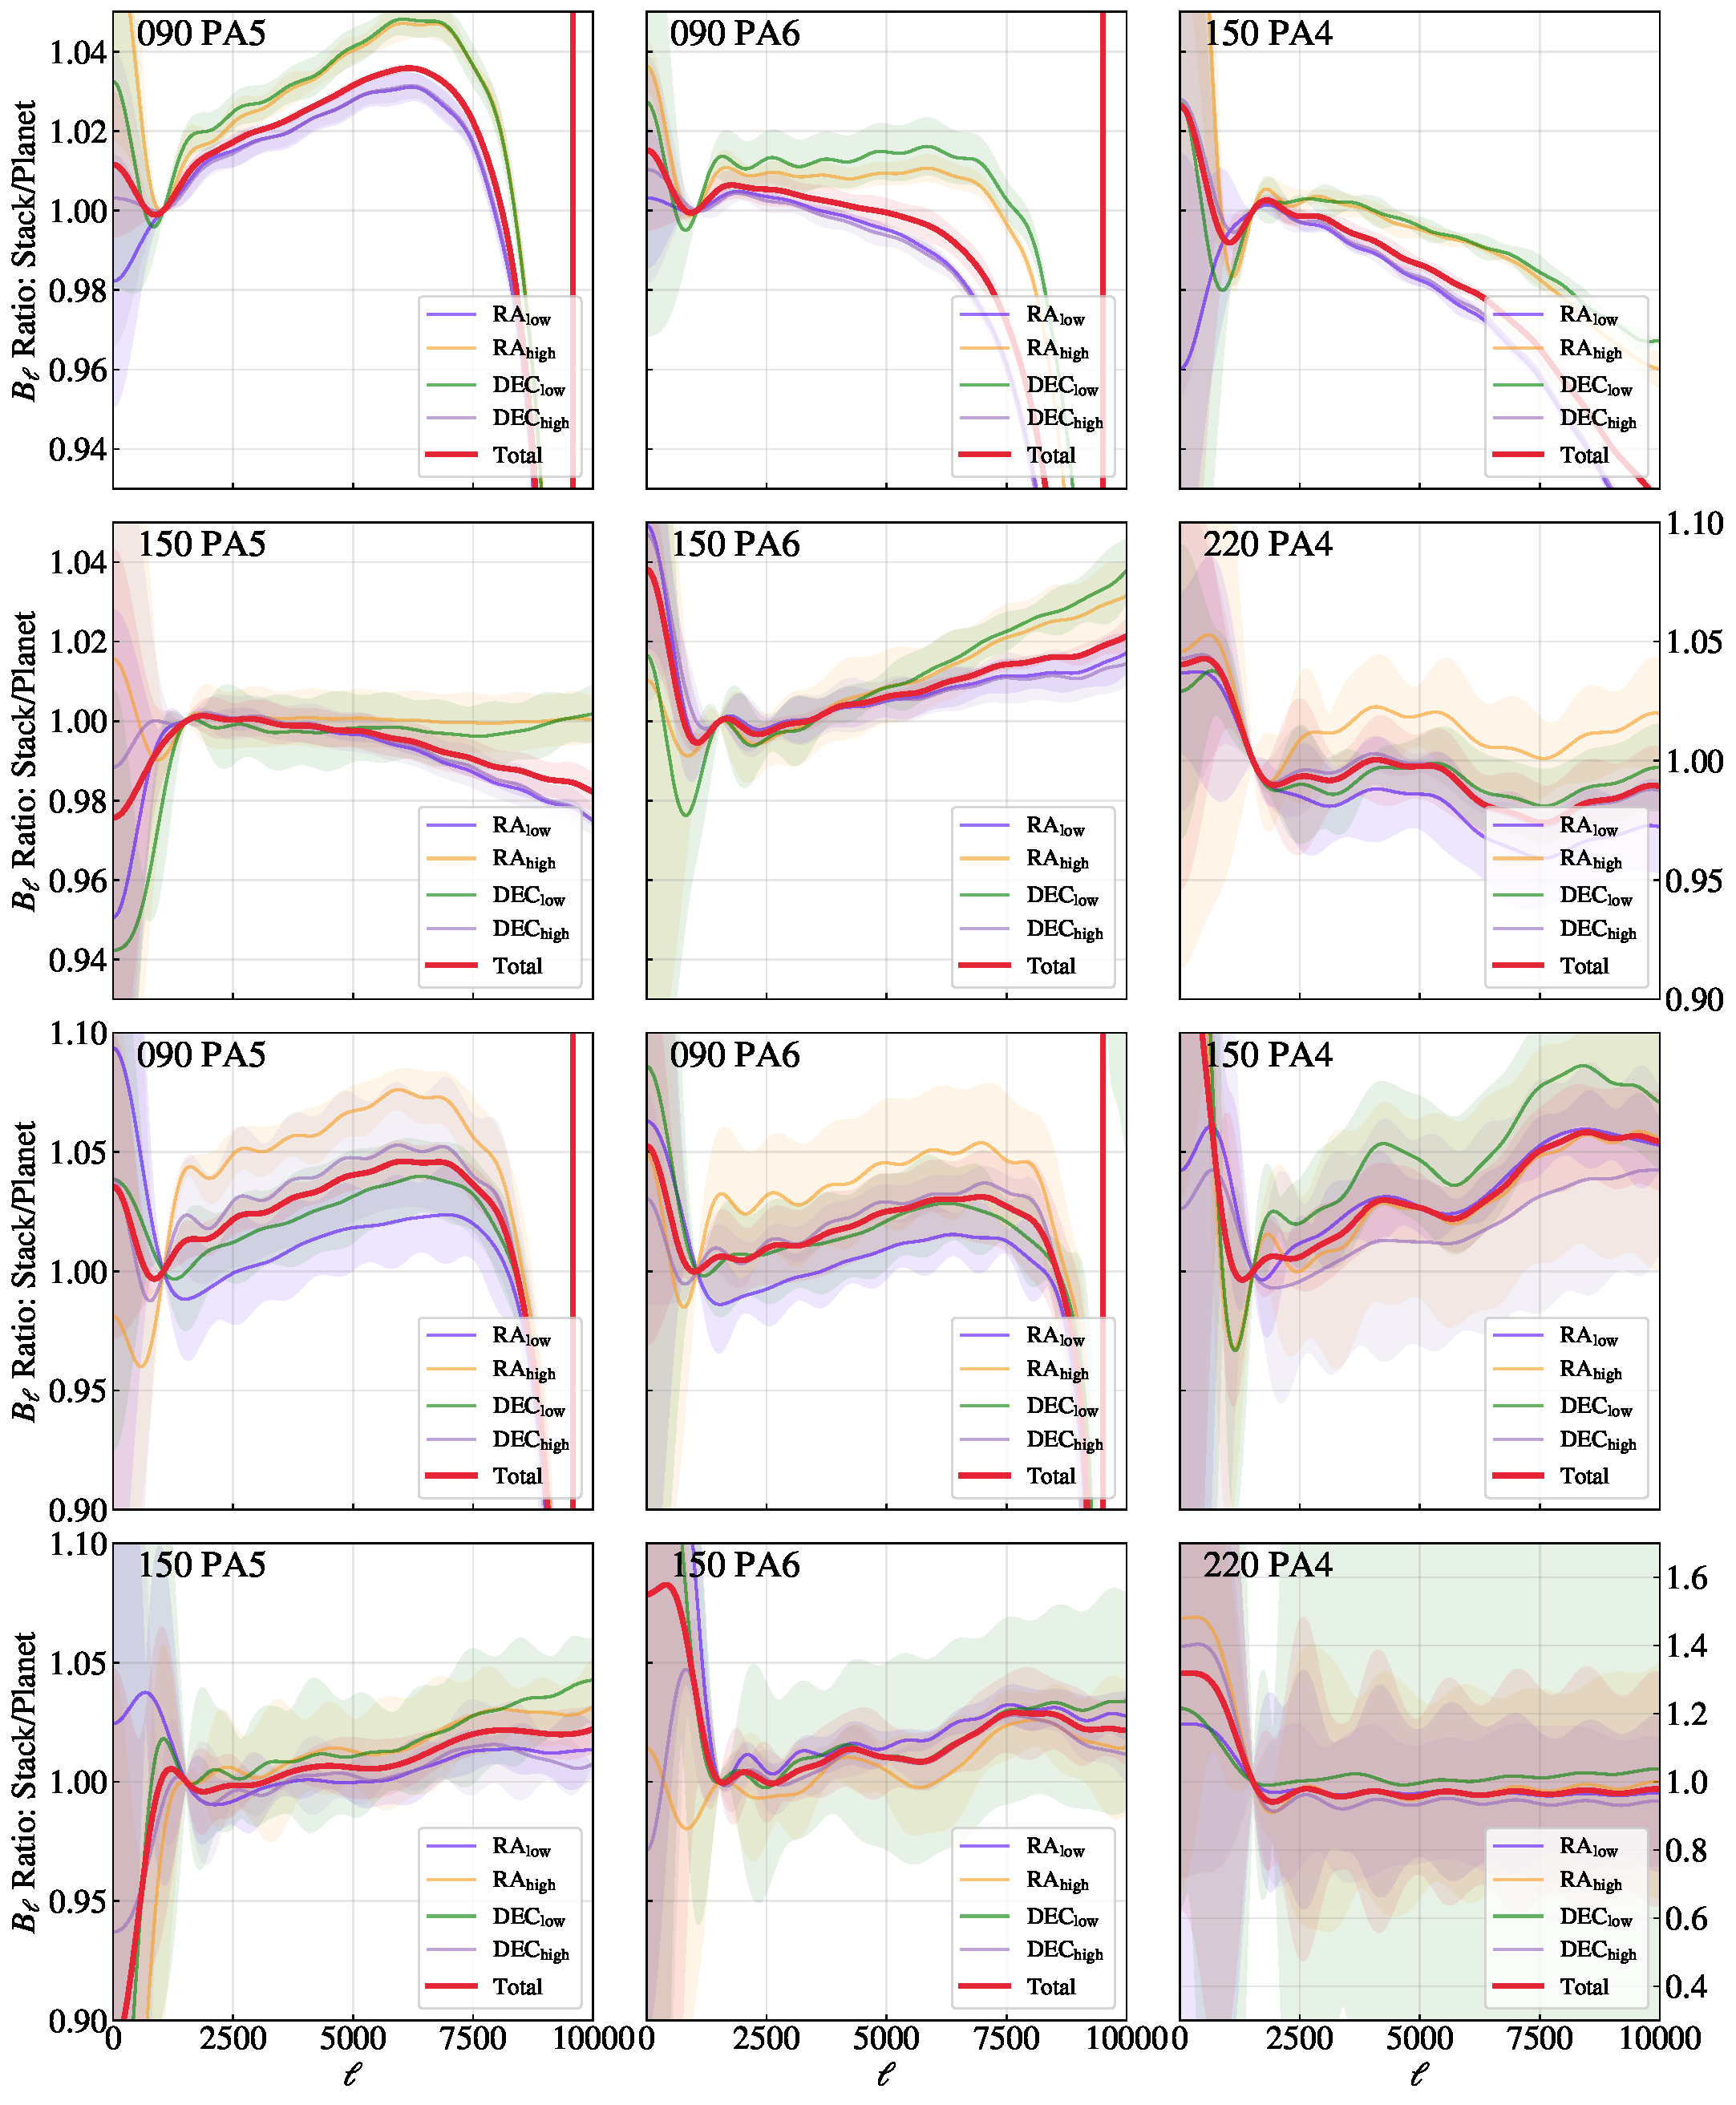
\includegraphics[width=.9\textwidth]{Figures/Bells_ratio_planet.png}
    \caption{Window function of stacked point sources, separated by RA and DEC, which we consider as a null test.  The full map stacked is plotted in red.}
    \label{fig:bells}
\end{figure*}

\subsection{Temperature to Polarization Leakage Beam}
\label{subsec:polbeam}
Here, we present the polarized beams of the stacked point sources to determine polarization leakage in the instrument. 
\begin{itemize}
    \item different polarization cut on point sources.
    \item figure with stacked QUEB, model QUEB, and residual QUEB.
    \item window functions of T$\xrightarrow[]{}$E and T$\xrightarrow[]{}$B, leakage.
\end{itemize}
The leakage is relatively small compared to the magnitude of the temperature beam, however the sensitivity of ACT DR6 data is such that this leakage needs to be accounted for in the analysis.  Previously, observations of Uranus were used to build an $\ell$-space T-to-P leakage function for a given frequency and array in the instrument.  Here, we test this method by comparing the leakage to our new method of stacking.
\begin{equation}
\label{eq:trans_e_b}
    \{\tilde{E}(\ell), \tilde{B}(\ell)\} = -2\pi\int \{\tilde{Q}_r(\theta),\tilde{U}_r(\theta) \} J_2(\ell\theta)\;\theta\;d\theta \; .
\end{equation}

\section{Discussion}
\label{sec:disc}
\subsection{Beam Products}
\label{subsec:prods}
\subsection{Conclusion}
\label{subsec:concl}
In this paper, we have presented the analysis of the ACT beams for DR6, which includes data from 2017--19. ...
